\documentclass[11pt]{article}

\usepackage{amsmath}
\usepackage{booktabs}
\usepackage{caption}
\usepackage{comment}
\usepackage{deauthor}
\usepackage{epsfig}
\usepackage{graphicx}
\usepackage{pgfplots}
\usepackage{pifont}
\usepackage{subfig}
\usepackage{times}
\usepackage{url}
\usepackage{wrapfig}
\usepackage{xcolor}
\usepackage{xspace}

%\graphicspath{{rogers/figs/}{../figs/}}
\renewcommand{\thesubfigure}{(\alph{subfigure})}





\newcommand{\shortsection}[1]{\vspace{0.2em}\noindent {\bf #1.}}
\newcommand{\mechanism}{$\mathcal{M}$\xspace}
\newcommand{\db}{$\mathcal{D}$\xspace}
\newcommand{\eps}{$\epsilon$\xspace}
\newcommand{\answer}{$\mathcal{R}$\xspace}
\newcommand{\query}{$\mathcal{Q}$\xspace}

\newcommand{\sandp}{S\&P\xspace}
\newcommand{\prover}{$\mathcal{P}$\xspace}
\newcommand{\verifier}{$\mathcal{V}$\xspace}
\newcommand{\zk}{ZK\xspace} %can change to "ZK" if we hit space constraints
\newcommand{\zkp}{ZK proof\xspace} %can change to "ZK proof" if we hit space constraints
\newcommand{\zkps}{ZK proofs\xspace} %can change to "ZK proofs" if we hit space constraints
\newcommand{\cut}[1]{}


\begin{document}

\title{Everything You Always Wanted to Know About\\ Secure and Private Database Systems (but were Afraid to Ask)}



\author{Donghyun Sohn, Xiling Li, Jennie Rogers\\
\{donghyun.sohn,xiling.li,jennie\}@northwestern.edu}


\maketitle


\begin{abstract}
Individuals and organizations are accumulating data at an unprecedented rate owing to the advent of inexpensive cloud computing.  Data owners are increasingly turning to secure and privacy-preserving collaborative analytics to maximize the value of their records. In this paper, we will survey the state-of-the-art of this growing area.   We will describe how researchers are bringing security and privacy-enhancing technologies, such as differential privacy, secure multiparty computation, and zero-knowledge proofs, into the query lifecycle.  We also touch upon some of the challenges and opportunities associated with deploying these technologies in the field.
\end{abstract}


\section{Introduction}


With the rise of inexpensive cloud computing and its highly available storage, we are collecting data at an unprecedented rate.    Businesses, governments, and other organizations are increasingly outsourcing their data management operations accordingly.  They are also realizing new opportunities for analytics in important domains such as clinical research, public policy, and more.  There are, however, (at least) two issues that prevent this burgeoning field from reaching its full potential. First, data owners are concerned about the security and privacy of outsourcing their private records, especially regarding their liability and compliance obligations.  Second, despite the ubiquity of data, records remain fractured among multiple independent databases.  Without putting data in context, these systems may produce query answers that are incomplete and misleading. 


To address these challenges, the database community has been very actively researching techniques that protect confidential records in a relational database by architecting security and privacy (S\&P) techniques as first-class citizens in their operations.  This is happening at every step of the query lifecycle, as shown in Figure~\ref{fig:pets-workflow}.  In this paper, we will look at systems that are {\em secure}; they protect their records from unauthorized access.  We will also describe ones that are {\em privacy-preserving}\textendash they release information about a dataset while protecting their individual records from reconstruction attacks.  We will also delve into outsourced {\em verifiable} systems, where an untrusted party provides authenticated query answers over private data.  These problems are partially overlapping and we refer to solutions in this space as  {\em trustworthy database systems}.  This myriad of \sandp options for databases might seem bewildering to newcomers.  In this paper, we will offer a field guide to these emerging systems.  We will describe their guarantees and outline the advantages and disadvantages to competing approaches.    

We organize the rest of this paper as follows. We review the fundamentals of trustworthy database systems in Section~\ref{sec:background}.  After that, we will survey the state-of-the-art for secure query processing in Section~\ref{sec:secure}.  We will then progress on to examine techniques for integrating differential privacy into the query processing pipeline in Section~\ref{sec:dp}.  After that we will describe techniques for verifiable query processing in Section~\ref{sec:verifiable}.  Last, we discuss how researchers are assembling these building blocks into privacy-preserving database operators in  Section~\ref{sec:ops}. 


\begin{wraptable}{r}{0.5\textwidth}
  \centering
  \vspace{-4mm}
    \begin{tabular}{c|l}
        Symbol & Meaning  \\
        \hline
        \query & A query submitted to a trustworthy DBMS\\
        \db & A database over which we evaluate \query \\
        \mechanism & The mechanism that computes \query \\
        \answer & The result of \query computed over \db\\
        $\mathcal{C}_{ver}$   & A checker for verifying \answer\\
    \end{tabular}
    \caption{Notation for query workflow}
      \vspace{-4mm}
    \label{tbl:notation}
\end{wraptable}




\section{Background}
\label{sec:background}



In this section, we review the fundamental concepts that underpin trustworthy database systems.  These systems are built upon several techniques from the security and privacy community.  They range from cryptographic primitives for protecting data at rest and during query evaluation to frameworks that quantify and control the information leakage associated with running a query.  %We outline them in the context of a generic query processing lifecycle in Figure~\ref{fig:pets-workflow}.
This survey will explore database systems that protect their records' privacy or integrity from one or more adversaries.  Systems that center on protecting the privacy of user queries, as opposed to private data, are beyond the scope of this paper.  Examples of this include private information retrieval~\cite{chor1998private, olumofin2010privacy}, searchable symmetric encryption~\cite{hacigumucs2002executing}, and private function evaluation~\cite{wang2017splinter}. % Similarly, we will not address blockchain systems~\cite{allen2019veritas, el2019blockchaindb} 





Early privacy-preserving database research  {\em anonymizes} private data~\cite{lefevre2005incognito, nergiz2008multirelational,machanavajjhala2007diversity,li2006t}.   For example, $k$-anonymity~\cite{sweeney2002k}  only releases a record, or aggregate thereof, if there are at least $k-1$ others  that are indistinguishable from it.   These techniques give the misleading intuition that individuals   ``hide in the crowd'' in an anonymized data release, but research indicates that the widespread availability of auxiliary data and reconstruction attacks makes this position unsustainable~\cite{narayanan2014no, ohm2009broken, rocher2019estimating}.  We touch upon anonymization here because, at the time of this writing, this approach enjoys regular use in numerous domains including US healthcare~\cite{office2002standards} and education~\cite{chicaiza2020application, seastrom2017best} data protection and we expect to see this continue in the near-term as more effective approaches mature and gain traction.   We will focus on these next-generation techniques in the remaining text.



\shortsection{Notation}  We outline the notation we will use in this text in Table~\ref{tbl:notation}.  Our query workflow begins with a client submitting their query, \query, to a trustworthy DBMS.  They wish to run this SQL statement against a private database, \db.  If they are querying $n$ private engines, they query ($\mathcal{D}_1$, \ldots, $\mathcal{D}_n$).  The client may or may not be trusted with the records of \db, as we will cover shortly.   The database evaluates the query with a mechanism, \mechanism, that produces its \sandp-preserving result, \answer := \mechanism(\db).  If we are accompanying \answer with a proof of its authenticity, then we compute a boolean function, $\mathcal{C}_{ver}(\mathcal{D}) \in \{0, 1\}$, and it returns {\tt 1} to the client if it verifies \answer successfully.



\begin{wrapfigure}{r}{0.5\textwidth}
\vspace{-4mm}
\centering
    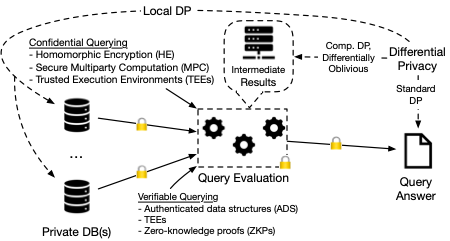
\includegraphics[bb = 0 0 220 118]{submissions/submission1/figs/pets-workflow.png}
        \caption{ Trustworthy DBs  in the query lifecycle}
    \label{fig:pets-workflow}
\end{wrapfigure}




\subsection{Query Lifecycle}

Figure~\ref{fig:pets-workflow} shows the broad steps with which a database system  evaluate a query and where they integrate assorted privacy and security-enhancing techniques into this workflow.  This figure is inspired by~\cite{secretflow2024survey}.  The dotted lines denote steps in the process that may leak information about a database's private records.  We expect  the initial input databases from one or more {\em data providers} or {\em data owners} are correct and complete at setup time.  A {\em clients} queries the records of one or more private databases.  The party computing the query answer\textendash this could be the data owner themselves, an untrusted cloud service provider used for outsourcing or others\textendash may have access to this information leakage.   We delve into specific trustworthy database architectures and the \sandp-preserving techniques that power them in the upcoming sections.    




\begin{figure}
\centering
    \subfloat[Client-Server]{
    \label{fig:arch:client-server}
    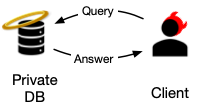
\includegraphics[bb= 0 0 113 65]{submissions/submission1/figs/client-server.png}}
    \hfill
    \subfloat[Outsourced Storage]{
    \label{fig:arch:outsourced-storage}
    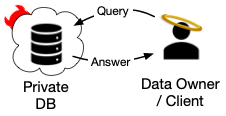
\includegraphics[bb= 0 0 113 65]{submissions/submission1/figs/outsourced-storage.png}}
    \hfill
    \subfloat[Private Data Federation]{
    \label{fig:arch:private-data-federation}
    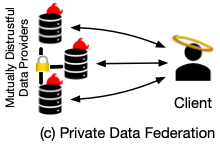
\includegraphics[bb= 0 0 113 65]{submissions/submission1/figs/private-data-federation.png}}  
    \hfill
    \subfloat[Outsourced  Computation]{
    \label{fig:arch:outsourced-computation}
    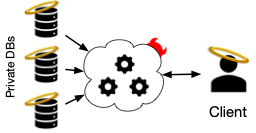
\includegraphics[bb= 0 0 113 65]{submissions/submission1/figs/outsourced-computation.png}}  
    \caption{Reference architectures for trustworthy database systems.}
    \label{fig:arch}
\end{figure}



\subsection{Trustworthy DBMS Architectures and Roadmap}
\label{sec:arch}

Throughout this text, we will reference several common architectures for query evaluation.  In this section, we will describe trustworthy database systems in terms of the  four architectures shown in Figure~\ref{fig:arch}. Our goal is to provide a  guide for future systems builders in selecting the most suitable one for their setting.  Admittedly, these frameworks are partially overlapping. We break them up as shown for ease of exposition.
 
A {\em client-server} architecture simply enables the client to send their  \query to the server with a private database and receive its answer, \answer as in Figure~\ref{fig:arch:client-server}.    For example, if the client is untrusted and the data provider is trusted, then the latter might protect their query answers from reconstruction by returning noisy versions of the true query answer using differential privacy.  We will cover this approach in Section~\ref{sec:dp}. 


The {\em outsourced storage} architecture, depicted in Figure~\ref{fig:arch:outsourced-storage}, starts with one or more untrusted cloud servers that have ample storage and limited compute resources. A data owner or trusted client outsources their storage operations to this platform to keep their data confidential.   These systems support a key-value store-esque interface. This is challenging because even when the database is stored encrypted, side-channel information such as memory access patterns can reveal some or all of the DB's contents~\cite{grubbs2016breaking,kellaris2016generic,markatou2019full}.  We introduce oblivious RAM in Section~\ref{sec:oram}; it is the main starting point for systems in this space.   If the client seeks only verifiable results, and they have access to more compute power on the server side,  they  might engage in verifiable querying as described in Section~\ref{sec:verifiable}.


The {\em private data federation} (PDF), shown in Figure~\ref{fig:arch:private-data-federation}, enables two or more mutually distrustful parties to compute \answer over the union of their private records without disclosing their private records to anyone.  This secure query evaluation may take place within cryptographic protocols evaluated among the data providers, described in Section~\ref{sec:oblivious} or in trusted hardware, as detailed in Section~\ref{sec:tees}.  


The {\em outsourced computation} setting in Figure~\ref{fig:arch:outsourced-computation} is when one or more data providers outsource their storage to the untrusted cloud and they delegate all query evaluation to this platform.  Here, the client and data providers are both trusted.  We discuss approaches to solving this challenge in Section~\ref{sec:secure}.  Similar to the PDF, platforms can securely compute in hardware or software.  This setup introduces another option: homomorphic encryption, or computing over encrypted data, as described in Section~\ref{sec:he}.

\section{Secure Query Processing}
\label{sec:secure}

In this section, we will examine techniques for query processing on outsourced databases, Figure~\ref{fig:arch:outsourced-computation}, and private data federations, Figure~\ref{fig:arch:private-data-federation}.   We group together these two architectures because there is strong overlap in their approaches and we highlight their differences we go along. We start with the strongest guarantee, oblivious querying, and then introduce popular relaxations to this. 

\subsection{Oblivious Querying}
\label{sec:oblivious}

A program is {\em oblivious} if its data access patterns and instruction traces are independent of their private input data.   \cut{An oblivious program's control flow does not change as a function of its private inputs.}  Oblivious algorithms prevent an attacker from inferring information about a database by observing its queries as they are evaluated.  An obliviously-executed query divulges nothing about its private inputs, except that which can be deduced from its results.

Researchers prove that a program is oblivious using the ``real world, ideal world'' paradigm~\cite{Canetti2001}.  Say that we are computing query  \query with mechanism \mechanism over database \db and there exists a probabilistic polynomial time simulator, $Sim$ that receives \db', an arbitrary database that is not \db but shares its schema and table cardinalities.   The observable traces of \mechanism should be computationally indistinguishable from those of $Sim$.  In other words, $Traces(\mathcal{M}, \mathcal{D}) \equiv Sim(\mathcal{M}, \mathcal{D}')$.  This paradigm makes it possible to compose independently developed building blocks, such as the oblivious query operators, into a query plan with strong end-to-end guarantees.  

There are a few common mechanics in oblivious database operators~\cite{bater2017smcql, zheng2017opaque,volgushev2019conclave,liagouris2023secrecy,ant2024scql}.  To keep their instruction traces oblivious to their private inputs, these programs evaluate both branches of private if-then statements, retaining only the one indicated by its secret conditional.  Similarly, they do not admit early termination of loops.  They conceal the selectivity of database operators with {\em dummy tuples} that replace rows that would be filtered out in an operator so that a curious observer cannot deduce anything  about a function's input data.  These engines typically represent this feature with a {\em dummy tag} or bit appended to each row  denoting whether it should be included in any subsequent calculations.  For example, an oblivious filter visits every row in a table and  applies its private predicate.   If the row satisfies the selection criteria, the oblivious if-then will update the row's dummy tag.  Otherwise,  it will simply overwrite the dummy tag with its previous value to remain oblivious.  We will describe oblivious database operators in detail in Section~\ref{sec:ops}.


Oblivious querying incurs a substantial performance penalty because its operators hide their data access patterns and any data-dependent changes in their control flow. With no additional info, queries with cascading joins must pad their output to the maximum possible size (the cross-product of their inputs) to conceal their selectivity.  Cumulatively, leads to a blow-up in their cardinalities increasing the cost of any subsequent computation.   As such, many oblivious database operators engage in selective information disclosure such as revealing the true cardinality of joins~\cite{krastnikov13efficient, zheng2017opaque} by default while offering full-padding  if desired.  If this is the root (last) operator in a query tree and the parties will receive \answer, then this is a sensible trade-off.  This picture gets more complicated if it is an intermediate result.


{\em Secure multiparty computation} (MPC)~\cite{goldreich1987mpc,lindell2021mpc} enables two or mutually distrustful parties to jointly compute over their private inputs obliviously.  Although early applied MPC protocols often implemented a special-purpose function (such as linear regression) to tackle the breathtaking overhead associated with general-purpose protocols, most modern systems compile their program logic into circuits~\cite{marcella2019sokmpccompilers}.  These {\em garbled circuits} reduce \query  into a series of gates, e.g., AND and XOR gates.  The protocol evaluates the circuit obliviously by traversing it in topological order.  They provide a Turing complete springboard for evaluating ad-hoc queries.   Some protocols use arithmetic gates instead of logic ones.   Performing all private computation within garbled circuits makes it possible to seamlessly compose the security guarantees of multiple, independently-developed components into a single proof under universal composability~\cite{Canetti2001}. 


\shortsection{Private Data Federations} There is a growing need to analyze information from multiple sources through a unified querying interface while addressing privacy concerns and complying with numerous privacy laws. A PDF, as  in Figure~\ref{fig:arch:private-data-federation}, integrates multiple autonomous database systems owned by mutually distrustful parties to query them as if they were a single query engine.  PDFs offer a shared schema that has table definitions agreed upon by all data providers at setup time.  It specifies the security level needed for each column.  Many PDF frameworks evaluate their queries under MPC.    This ensures that no unauthorized data is disclosed to other data providers participating in a secure query, while also minimizing the operations that \mechanism must perform under MPC by pushing them down for local evaluation~\cite{bater2017smcql, volgushev2019conclave, liagouris2023secrecy}.  


Data providers store private data in their own databases and compute query outputs in a privacy-preserving manner.  In PDFs, the process operates as follows: the client translates \query into the corresponding cryptographic protocols with which they will execute it.  They then send these instructions to all participating data providers.  The data providers then locally compute any public query operators  over their private records.  They then encode their selected private input rows for the operators that require secure, distributed evaluation over their unioned intermediate results.  They execute their oblivious operators by passing encrypted messages among themselves.  The data providers then send their share of \answer to the client over an encrypted link.  After receiving shares from all of the computing parties, the client assembles \answer. 

There are numerous threat models for MPC protocols, and they are detailed in~\cite{lindell2021mpc}.    A {\em semi-honest} party adheres to the protocols, but may attempt to learn additional, unauthorized information from observing the MPC protocol.  Semi-honest database systems include SMCQL~\cite{bater2017smcql}, Conclave~\cite{volgushev2019conclave}, and Hu-Fu~\cite{tong2022hu}. On the other hand, a {\em malicious} party both seeks to reveal information about a query's private inputs and they may deviate from the MPC protocol arbitrarily.  Senate~\cite{poddar2021senate} implements a PDF in the maliciously secure setting.  Some engines are starting to support multiple protocols or mixed models by compiling queries into abstract circuits (or methods) and applying different protocols for different settings.  SCQL~\cite{ant2024scql} and VaultDB~\cite{rogers2022vaultdb, vaultdb} take this approach.  Naturally, protocols with stronger guarantees incur more overhead for query evaluation, and this design choice depends on the setting in which they run.

\shortsection{Outsourced Computation}  MPC facilitates querying over the unioned data of 2+ independent private DBs.  We need one more step to extend this technology to the outsourced computation setting in Figure~\ref{fig:arch:outsourced-computation}.  To distribute trust over multiple outsourced hosts, a client may  {\em secret share} their private inputs and send shares of them to all computing parties.  Here no  party can reconstruct the secret unless the party colludes with a subset of parties. Before starting to evaluate \query's garbled circuits,  the parties participate in an {\em oblivious transfer} protocol to encode their data as wire labels for its logic gates.   This process is analogous to public-key cryptography where at the end of it each party holds an encrypted copy of the database without access to the key with which to decrypt it and none has access to the plaintext data except its initial owner.   


Platforms in the outsourced computation model have also been adopting MPC protocols.  The earliest work (to the best of our knowledge) in this space computed aggregates semi-honestly under 3-party computation~\cite{bogdanov2008sharemind}.  SDB~\cite{wong2014secure,Zhian2015SDB} created a hybrid model where the private data is secret-shared among the data owner and the cloud service provider.  For the semi-honest setting, Secrecy~\cite{liagouris2023secrecy} supports 3-party secure computation over ad-hoc SQL queries.     RESCU-SQL~\cite{li2023rescu} uses maliciously secure, $n$-party MPC protocols to protect outsourced data in the zero-trust cloud.  




\subsection{Oblivious RAM for Outsourced Storage}
\label{sec:oram}

We now turn our attention to the outsourced storage setting shown in Figure~\ref{fig:arch:outsourced-storage} in Section~\ref{sec:arch}.  Here, the client wishes to outsource the of their private database to the untrusted cloud.  If they simply encrypted their data and issued read and write requests against the specific records as they access them, then this will expose their data access patterns and make their data vulnerable to side-channel leakage attacks~\cite{kellaris2016generic, naveed2015inference, grubbs2016breaking}.  Unless otherwise specified, these systems have a key-value store-style API.   {\em Oblivious RAM}~\cite{goldreich1987oram} transforms a client's read and write requests into ones that are independent of their true memory access patterns. When a client requests a block, $b_i$, from their database, the ORAM rewrites it as a series of reads and writes that 1) shuffle their storage, and 2) pad their request with dummies to conceal the position of their request in the database.    This makes the distribution of their I/O requests oblivious to their true memory access patterns.  It also prevents an adversary from deducing the frequency of accesses to a specific $b_i$.  

Early work in outsourced storage centered on ORAM constructions themselves, with tree-based ones~\cite{stefanov2013pathoram, ren2015constants} emerging as the dominant paradigm in practice.  Several systems have generalized this work to distributed ORAMs, including Shroud~\cite{lorch2013shroud}, ObliviStore~\cite{stefanov2013oblivistore}, and TaoStore~\cite{sahin2016taostore}.  Snoopy~\cite{dauterman2021snoopy} integrates trusted hardware into their design to parallelize oblivious reads and writes.   Whereas ORAM makes all access requests indistinguishable from one another,  {\em frequency smoothing} relaxes this requirement to make the frequency with which individual $b_i$s are requested uniform.  Waffle~\cite{maiyya2023waffle} and Pancake~\cite{grubbs2020pancake} are examples of this approach. They do so by replicating popular objects and padding their I/O requests with dummies. 


The systems described above are all linearizable; they reason about concurrency at the granularity of one object at a time.  Additional mechanisms are needed for ACID transactions.   Obladi~\cite{crooks2018obladi} is an ORAM-backed storage engine that parallelizes ACID transactions on untrusted ORAM servers.  Treaty~\cite{giantsidi2022treaty} is a natural extension of this work obviates the need for a trusted proxy with trusted hardware.


\subsection{Homomorphic Encryption for Outsourced Computation}
\label{sec:he}

{\it Homomorphic encryption} (HE)~\cite{gentry2009fully} enables a system to compute over encrypted data without decrypting it.    HE and MPC are close cryptographic cousins.  Rather than distributing trust over multiple parties, HE enables data owners to outsource their operations to one host with a variation of the outsourced computation architecture in Figure~\ref{fig:arch}.  Here, the data provider encrypts their records and uploads them to the untrusted cloud (without providing the decryption key) and the client issues queries against the encrypted databases.   Whereas MPC enables parties to pipeline their circuit evaluation, i.e., compute each gate and discard intermediate wire labels when they are no longer needed, HE protocols evaluate a materialized circuit to produce \answer and send it to the client.  This is more efficient for straightforward operators such as filter, but may reveal scalability challenges for ones with deeper circuits such as aggregating over a large group of tuples.  Fully homomorphic encryption (FHE)  support circuits, and thus ad-hoc queries, without leaking information about the encrypted data.  FHE has a very high performance cost, typically several orders of magnitude slower than running in plaintext.  These schemes have seen limited adoption in databases in practice with the only known implementation for databases targeting aggregation alone~\cite{ren2022heda}.  HE has several relaxations to bridge this performance gap.  Some partially homomorphic encryption (PHE) schemes offer better performance in exchange for reduced security guarantees, such as order preserving encryption~\cite{boldyreva2009order,agrawal2004order} and deterministic encryption~\cite{boldyreva2008notions, bellare2008deterministic}.  Others support reduced expressiveness with higher performance, such as additive HE~\cite{paillier1999public} and multiplicative HE~\cite{elgamal1985public,rivest1978method}.

Database researchers have invested substantial research effort into bringing these encryption schemes to outsourced databases with a variation of the architecture in Figure~\ref{fig:arch:outsourced-computation}.  The data owner encrypts \db using HE and uploads them to the untrusted cloud server.  The client submits \query to the server and it computes \answer over its encrypted copy of \db.  ~\cite{agrawal2004order} introduced order-preserving encryption for answering database queries.  CryptDB~\cite{popa2011cryptdb}
and Monomi~\cite{tu2013processing} targeted HE for outsourced databases for OLTP and OLAP workloads, respectively.  The latter identified lightweight mechanisms for moving some of the query evaluation client-side to circumvent the performance limitations of FHE.  Unfortunately, these PHE schemes have substantial side-channel leakage associated with executing queries over them~\cite{naveed2015inference, bindschaedler2017tao}.  This is similar to the issues we described for non-oblivious access to outsourced storage above.  SEAL~\cite{demertzis2020seal} tackles some of this leakage with adjustable leakage that hides $\binom{n}{k}$ bits out of a search key by introducing a generalization of ORAM.


\subsection{Trusted Execution Environments for Outsourced and Federated Querying} 
\label{sec:tees}

Trusted Execution Environments, or TEEs, create an isolated computing platform within an untrusted computer using trusted hardware.  They have encrypted private memory with which they runs sealed code that is confirmed to be only the code given by the client or a proxy thereof (such as a trustworthy DBMS).  Hence, code run within TEEs are verifiable by virtue of running within a secure enclave, such as Intel SGX~\cite{dinh2019everything} and ARM TrustZone~\cite{pinto2019demystifying}.   Clients  delegate their program executions to trusted hardware, safeguarding their private data without the need for encryption. The main advantage is its efficiency, as it avoids the significant computational and communication overhead typically incurred by cryptographic primitives, making it more practical for real-world scenarios. Secure enclaves alone are not a panacea. For example, instruction traces leak memory access patterns, allowing eavesdroppers to infer private data from them~\cite{kellaris2016generic,markatou2019full}.

TEEs are seeing increased use for evaluating queries over confidential data  the cloud or outsourced computation in Figure~\ref{fig:arch:outsourced-computation}.  First-generation systems relied on software-hardware co-design to build TEEs with bespoke algorithms for query evaluation such as TrustedDB~\cite{bajaj2011trusteddb} from IBM and Microsoft's Cipherbase~\cite{arasu2013orthogonal}.  As SGX and other enclaves became widely available and cloud-ready, researchers created secure enclave extensions to well-known DBMSs.  For example, StealthDB~\cite{vinayagamurthy2019stealthdb} builds atop PostgreSQL and EnclaveDB~\cite{priebe2018enclavedb} runs within Hekaton.  In addition, since the resident host running the enclave can observe its memory access patterns, researchers have been building oblivious algorithms for use inside the TEE such as ObliDB~\cite{eskandarian2019oblidb} and Opaque~\cite{zheng2017opaque}.  This approach has also been appearing in TEE-based PDFs such as~\cite{dave2020oblivious}. 





\section{Differential Privacy} 
\label{sec:dp}

If the client is untrusted, the data provider may call for guarantees that prevent them from using query answers to infer information about their private input records. Speaking informally, {\em Differential Privacy} (DP) ~\cite{dp2006, dwork2008differential} protects private data from construction attacks by injecting carefully calibrated noise into their query answers to control their resulting information leakage before returning them to the client.   An algorithm satisfies differential privacy if its output is approximately the same over a database, \db, as it would be over a neighboring database differing by one record, \db'. This workflow, of a data provider or trusted curator noising query answers before releasing them to the client, is known as {\em Standard DP} or SDP~\cite{wagh2021dp}.     More broadly, if a secure database reveals precise, un-noised query answers, this creates unbounded information leakage~\cite{kifer2011no}.  SDP works on the client-server model in Figure~\ref{fig:arch:client-server}. 

Before answering their first query over \db, the data owner selects a privacy budget, \eps, with which they limit the information they leak in aggregate to the client or clients by answering their queries.  Recall that $\mathcal{R} := \mathcal{M}(\mathcal{D})$.   In its simplest form, if the client queries a private database $n$ times with mechanisms $\mathcal{M}_1, \ldots, \mathcal{M}_n$, and $\mathcal{M}_i$ has $\epsilon_i$, their net privacy loss is $\sum_{i=1}^n \epsilon_i$.  Researchers have proposed several frameworks for designing efficient DP mechanisms~\cite{johnson2020chorus, zhang2018ektelo, wang2021dpgen}.  Also, the database community has invested significant research effort into automatically deriving SDP answers to SQL queries with robust e2e  privacy guarantees ~\cite{ann2011airavat,mcsherry2009privacy,proserpio2014calibrating,johnson2018towards,kotsogiannis2019architecting, kotsogiannis2019privatesql}.



Choosing \eps for a given database and query workload reveals a trade-off between utility and privacy.  A larger \eps means that \mechanism will inject less noise into \answer.  In other words, more accurate query answers result in a greater privacy loss for \db.   Selecting an \eps with sufficient data protection while producing useful query answers is a challenging topic~\cite{lee2011much} and the subject of ongoing research~\cite{dwork2019differential, li2023towards, near2023guidelines}.  A conservative heuristic is to restrict $\epsilon$ to values less than or equal to one~\cite{wood2018differential}.

\subsection{Computational Differential Privacy} One major shortcoming of SDP is that assumes there is a single trusted data curator noising \answer.   \cut{It is attractive because its guarantees are information-theoretic.}  Computational DP (CDP)~\cite{beimel2008distributed, mironov2009computational} relaxes SDP's strong information-theoretic guarantees to a weaker, probabilistic polynomial time adversary in exchange for less noisy results and support for distributed data.   CDP quantifies information leakage when two or more parties are computing a function over their encrypted and unioned private inputs, $\mathcal{D}_*$.    It frames information leakage about \mechanism's intermediate results as a differentially private view of $\mathcal{D}_*$ and assigns some share of the privacy budget to it.    For example, if we are computing a CDP filter $\mathcal{R} := \sigma(\mathcal{D})$ we may start by running the oblivious evaluation described above.   We then generate a noisy version of its true output cardinality {\em within} the oblivious algorithm for release, $|\widetilde{\mathcal{R}}|$ and obliviously delete dummy rows.  This will make any parent operators run faster because they compute over fewer dummies. 

CDP introduces a third dimension to our DP trade-off:  performance.
If we allocate more privacy to computation, the client may get their query answer faster but with reduced accuracy because we spend some privacy releasing information about \mechanism's intermediate results, i.e., its noisy intermediate cardinality.  There's been significant research interest in using CDP to accelerate privacy-preserving query evaluation in PDFs~\cite{bater2018shrinkwrap, bater2020saqe,he2017composing}. 


CDP  extends to the outsourced storage setting.  Allowing an untrusted cloud service provider to view noisy versions of the client's memory access patterns enables this trade-off on efficiency and privacy.   DP-ORAM~\cite{wagh2018differentially} relaxes ORAM's full-oblivious guarantees to CDP ones.    $\epsilon$psolute~\cite{kellaris2017accessing, bogatov2021varepsilonpsolute} parallelizes CDP I/O requests among multiple ORAMs.   CDP has also been used to speed up outsourced computation for analytics~\cite{roy2020cryptepsilon} and for querying growing databases~\cite{zhang2023longshot, wang2022incshrink,wang2021dp} in the untrusted cloud.  



\subsection{Differential Obliviousness}
 Another DP relaxation gaining traction in the database community is differential obliviousness~\cite{chan2022foundations,chu2021differentially, qin2022adore, qiu2023doquet} (DO).   A DO algorithm offers a DP view of its memory traces by leaking approximate versions thereof.   This is related to CDP, with the latter approximating discrete views of \db.  To continue with our filter running example, a simplified version of the DO filter in~\cite{qin2022adore} partitions \db into batches of length $B$ where $B$ is polylog of $|$\db$|$. In lieu of running an oblivious filter, it writes to the output buffer of \answer one batch at a time maintaining a cursor for these writes.  For each block $b_i$ it computes a DP approximation of its prefix sum (how many rows are selected), this provides a range of the count of the rows $b_i$ will emit to \answer.  It then writes to $B$ slots in the output buffer with a mix of real and dummy rows and advances the cursor to the position indicated by the lower bound of its DP prefix sum. 
 
 DO strikes a balance between full-oblivious ones and ones with unbounded information leakage.   It admits secure algorithms with performance properties comparable to streaming or pipelined operators and it boasts better cache efficiency than approaches that materialize their entire \answer before noising it.     On the other hand, DO mechanisms are non-trivial compose~\cite{zhou2023theory}, and they need to maintain the notion of neighbor-preserving differentially oblivious datasets between an operator's input and output relations to compose a DAG of them.  Addressing this challenge is a topic of ongoing research.

\subsection{Local Differential Privacy}

  One more approach to limiting information leakage from querying private data is injecting noise into the private data before querying it.  Local DP~\cite{xiong2020comprehensive} (LDP) removes the need for a trusted data curator by noising it one row at a time.  There has been considerable research in incorporating this into database operations~\cite{cormode2018privacy,gu2019supporting,roth2020orchard,wang2017locally,xu13collecting}.  This is different from DP synthetic data generation~\cite{cai2023privlava,ge2021kamino,machanavajjhala2008privacy}, which creates a new dataset with values that mimic the distribution of a private one.  


LDP is attractive for aggregating ``wisdom of the crowd'' statistics, such as collecting new words and phrases for auto-complete as they enter the popular lexicon and identifying software bugs from noisy bug reports.  It also frees data collectors from the liability of storing raw user data, which may garner subpoenas or attempts to steal it.  Also, since the data are noised upfront,  clients may query it as many times as they wish without eroding the privacy budget.  On the other hand, because the data are perturbed one row at a time, the algorithm needs to add $O(\sqrt{n})$ to each entry for $n$ individuals contributing to \db, whereas SDP would simply noise the true count independent of the participant count~\cite{wagh2021dp}.




\section{Verifiable Querying}
\label{sec:verifiable}

Data owners are increasingly outsourcing their data management to the untrusted cloud.   With {\em verifiable computing} when an untrusted server answers a client query \query with \answer over a private database \db, they participate in a protocol to convince the client (with high probability) that \answer is correct and complete.   Here we have two participants: a prover \prover, the cloud service provider, and a verifier \verifier, the client.   If $\mathcal{C}_{ver}(\mathcal{D})$ is a function with which \prover and \verifier authenticates $\mathcal{R}$ with the following guarantees:
\vspace{-0.2cm}
\begin{itemize}
    \item Completeness.  If \prover faithfully executes \query then $ \mathcal{C}_{ver}(\mathcal{R})=1$.  \prover accepts honest proofs.
    \vspace{-0.3cm}
    \item Soundness.  If \prover outputs an incorrect \answer,  $Pr[\mathcal{C}_{ver}(\mathcal{R})=1] \leq \epsilon$, where $\epsilon$ is a negligible probability.
\end{itemize}
\vspace{-0.2cm}
Systems such as IntegriDB~\cite{zhang2015integridb}, Concerto~\cite{arasu2017concerto}, CorrectDB~\cite{bajaj2013correctdb}, VeriDB~\cite{zhou2021veridb} and vSQL~\cite{zhang2017vsql} use VC to guarantee data integrity for querying.  


There are several approaches to creating verifiable query answers.  With an {\em Authenticated Data Structure}, \prover generates a proof that accompanies \answer to validate that it is complete and sound.  The two main methods that instantiate ADS are tree-based and signature-based methods.  The tree-based method builds a binary tree for a database, where each leaf node stores a digest about tuples in the database, and its internal nodes are digests that summarize its children.   When evaluating a query, the database sends the query answer along with a set of digests for the relevant nodes to the client, who has the digest of the root node, to verify the answer by reconstructing the path to match the root node. IntegriDB is such a system that applies a dynamic tree-based ADS tailored for a specific set of queries, allowing the client to query and verify $\mathcal{R}$ using precomputed digests aided by the accompanying proof. On the other hand, signature-based methods constructs a set of signatures for tuples in the database. During query evaluation, the cloud-hosted database sequentially collects a set of signed tuples that it accesses. Then the client verifies each tuple that no unwanted tuple is included and no necessary tuple is missed.

Similarly, Concerto, CorrectDB and VeriDB utilize ADS-based verifiable computing to verify their queries, but they compose ADSs with TEEs benefit from greater efficiency than working solely with cryptographic primitives (see Section~\ref{sec:tees}). Concerto is a concurrent key-value store, while VeriDB and CorrectDB support ad-hoc SQL queries for relational databases.

With {\em interactive proofs}~\cite{zhang2015integridb}, \prover and \verifier  work together to confirm the authenticity of  a statement $C(w)$ over a witness $w$ via multiple rounds of challenge-response messages, thereby incrementally ensuring correctness and soundness.  This VC approach is an alternative to ADS.  Similar to MPC, these proofs work in the circuit paradigm\textendash they express their logic as gates. In our context, $w$ is the private database $\mathcal{D}$.  \prover and \verifier interactively establish $w$ as a commitment of \db.  This forms the immutable starting point for \prover's proof for \query. Upon receiving the last respone $\mathcal{R}$ from \prover, \verifier accepts it iif $\mathcal{C}_{ver}(\mathcal{R})=1$. In other words, \verifier rejects immediately if it receives any unconvincing response from \prover during the interaction. In contrast to ADS-based systems mentioned above, vSQL is more expressive by supporting a wider range of SQL queries through IPs. Although interactive proofs incur significant communication overhead between the client and server, vSQL operates with nearly the same efficiency as those systems.

However, the client might attempt to obtain extra information that it is not authorized to access. For example, VC-backed systems with ADS and interactive proofs ensure the integrity of an outsourced database, but they reveal the data owner's records to the cloud service provider. Moreover, TEE-based systems may leak memory access patterns through program traces, as discussed in Section~\ref{sec:tees}. Therefore, the aforementioned systems are inadequate to protect private data on an untrusted server. For this we need to add one more guarantee to our stack, {\em zero knowledge}~\cite{goldreich1991zkp,goldwasser1985zkp}:
\vspace{-0.2cm}
\begin{itemize}
    \item Zero knowledge. If  $\mathcal{C}_{ver}(\mathcal{R})=1$, \verifier learns nothing other than the fact \answer was computed correctly.
\end{itemize}
\vspace{-0.2cm}
To provide such a stronger guarantee in verifiable querying, the database community has adopted {\it zero-knowledge proofs} for SQL queries~\cite{zhang2017vsqlzk, li2023zksql} to offer privacy and confidentiality for query answering.  This guarantee is similar to the one we saw for obliviousness: \verifier learns nothing more than \answer and that which can be deduced from it.  The main difference here is that \prover is able to prove  properties of intermediate query results, such as proving a sorted list of tuples is monotonically increasing, rather than evaluating the entire program logic in circuits. Overall, \zkps enable \prover to convince \verifier of the query answer \answer by authenticating it with a proof, without revealing any additional information beyond the information that could be derived from \answer. This means we could simultaneously address both data integrity and data privacy for the outsourced database.



There are two main flavors of zero-knowledge proofs: {\it interactive} and {\it non-interactive} \zkps.  Interactive ones are analogous to MPC, where \prover and \verifier verify a circuit one gate at a time using pipelined gates. In contrast to IPs, \zkps divulges no additional information about $w$ beside the truth of $C(w)$ to \verifier while IPs do not hide $w$ from \verifier.

Zero-knowledge extension of vSQL~\cite{zhang2017vsqlzk} and ZKSQL~\cite{li2023zksql} utilize interactive \zkps. While the former remains theoretical as a pioneering effort, ZKSQL optimizes computationally expensive operators for practical use, such as sort and join, reducing their respective complexities from $O(n \log n)$ and $O(n^2)$ to $O(n)$. This optimization is achieved through \prover's local computation and interactive verification with ZK set operations, where the set-based proofs are represented by polynomials instead of circuits, unlike conventional interactive \zkps. For example, in sorting, we can only check if the result contains the same tuples as the unsorted table using ZK set equality when the result confirms to be monotonically increasing or decreasing.

Conversely, non-interactive ones construct a monolithic circuit for their query in a single step, providing a single proof that \prover sends with \answer. They require no additional interaction between \prover and \verifier and are widely used in blockchain applications. However, a significant drawback is the large proof size, which can be memory-intensive due to the one-shot construction. Despite potentially being more efficient than the interactive ones due to reduced communication overhead, we do not recommend this approach for systems aiming to scalability.

In addition to the single prover-verifier system, there are also distributed or decentralized verification systems that build atop blockchains~\cite{el2019blockchaindb, allen2019veritas, peng2020falcondb,yueglassdb}. They guarantee auditability, accountability, and traceability on the ledger during data sharing across mutually distrustful parties, but their combined records are largely accessible to all participants on the chain thus they are beyond the scope of this paper.

\section{Privacy-Preserving Database Operators}
\label{sec:ops}

This section introduces privacy-preserving database operators.  They are crucial for secure and privacy-preserving query evaluation. 


We start with oblivious operators.  Recall from Section~\ref{sec:oblivious} that they guarantee that their memory access patterns and program traces do not disclose any information about their private inputs.   These operators ensure that even if an adversary knows \query and observes its execution under \mechanism, they learn no additional information from participating in its evaluation.~\cite{arasu2014oblivious} introduced the earliest formal definitions for efficient algorithms for oblivious query processing.  This paper covers approaches for selections, joins, and group-by aggregation.  It was designed for use in TEEs, although no practical implementation of its results are forthcoming.  Since then, there has been a lot of excitement in the research community about creating efficient, oblivious algorithms for database operators~\cite{ant2024scql, bater2017smcql, krastnikov13efficient, zheng2017opaque}.  We will also touch upon operators that offer alternative privacy guarantees, such as CDP and DO from Section~\ref{sec:dp}.  We will mainly focus on joins in this survey because, in our experience, these tend to be the bottleneck for most secure query workloads.  In addition, joins have attracted the most research results to date in terms of operator algorithms proposed.

\subsection{Joins}

Table~\ref{tbl:joins} presents a comprehensive categorization of privacy-preserving join approaches. This considers several key dimensions: computational complexity, employed methods, type of leakage, number of participating parties, and supporting join types. Notably, the table organizes the joins based on their leakage, establishing distinct categories for oblivious joins, differentially oblivious joins, and differentially private joins. 


\begin{table}
    \centering
    \begin{tabular}{l|c|c|c|p{2.8cm}|c}
     {\bf Strategy}    & {\bf Complexity} &{\bf  Compute Method} & {\bf Leakage}  &{\bf  \# of Parties} & {\bf Join Type} \\
     \hline 
     Nested Loop & $O(n^2)$ & SH-2PC & Oblivious & 2:~\cite{bater2017smcql, vaultdb} & all \\
     
      &  &  SH-3PC & Oblivious  &  3:~\cite{volgushev2019conclave, liagouris2023secrecy} &  \\

      &  &  Mal-MPC & Oblivious  &  N:~\cite{li2023rescu} &  \\
     
      &  &  SH-2PC &   CDP &  2:~\cite{bater2018shrinkwrap, bater2020saqe} &  \\
       &  & TEE & Oblivious &  1:~\cite{li2008privacy}, $\geq2$:~\cite{dave2020oblivious}&  \\
       
     \hline
     NLJ w/semi-join & $(n \times RF)^2$ & SH-2PC & Oblivious & 2:  \cite{bater2017smcql}  & equi-join \\ 
    &  &SH-3PC  &  Oblivious  &  3:~\cite{chu2021differentially, liagouris2023secrecy} & \\ 
     \hline

    Index NLJ & $n \log ^2 n$ & ORAM & Oblivious & N:  \cite{chang2022towards}  & all \\ 
    \hline

    Sort-Merge Join & $n \log ^2 n$ & TEE & Oblivious & $\geq 1$: \cite{krastnikov13efficient, eskandarian2019oblidb, zheng2017opaque} & equi-join \\ 
                    &    & SH-3PC & Oblivious & 3:~\cite{li2024experimental} & \\
                    &    & TEE & DO & $\geq 1:$  \cite{chu2021differentially}& \\
                    \hline 
       PK-FK SMJ             & $n \log n$   & TEE & DO & $\geq 1$:~\cite{qin2022adore} & 1:n \\
     \hline
    
     Hash Join & $n$ & SH-3PC & Oblivious& 3:~\cite{mohassel2020fast} & equi-join \\ 
     \hline

     Hash SMJ & $n$ & SH-3PC & Oblivious& 3:~\cite{luo2024secure} & equi-join \\ 
     \hline

     PSI join & $n$ & SH-2PC & Oblivious & 2:~\cite{raghuraman2022blazing, wang2021secure}; & pk-pk \\
      & & Mal-2PC & Oblivious & 2:~\cite{raghuraman2022blazing} & pk-pk \\
      & $n \log n$  & SH-MPC & Oblivious & N:~\cite{ant2024scql} & equi-join \\
      & $n \ln \ln n$  & SH-MPC & CDP & N:~\cite{narayan2012djoin} & equi-join \\
      \hline
      
      Partition Join & $n \log ^2 n$   & TEE & Oblivious & N:~\cite{li2023soda} & equi-join \\
      & $n \log n$   & TEE & DO & $\geq 1$:~\cite{qiu2023doquet} & equi-join \\
    \end{tabular}
    \caption{Comparison of secure join algorithms.   }
    \label{tbl:joins}
\end{table}


\shortsection{Oblivious Join}
The most strict technique is fully oblivious join, which allows combining data from different sources without revealing sensitive information. Various algorithms have been evaluated in~\cite{li2024experimental} to determine their efficiency and security, as shown in table~\ref{tbl:joins}. The study reveals the overall efficiency ranking, wherein PSI emerges as the most efficient, followed by hash approaches. However, the efficiency of NLJ and SMJ can surpass others under high join selectivity. Additionally, optimal join order significantly improves efficiency, highlighting the importance of cost-based query optimization. 

\shortsection{DO Joins}
To improve efficiency, DO join permits a controlled degree of information leakage about the data while still providing meaningful privacy guarantees based on the relaxed notion of $(\epsilon, \delta)-$differential obliviousness. Key advancements in this area include the DO join~\cite{chu2021differentially}, Adore~\cite{qin2022adore}, Doquet~\cite{qiu2023doquet}, as shown in Table~\ref{tbl:joins}. Fully oblivious join algorithms are inefficient due to worst-case padding, resulting in significant performance overheads. The DO join algorithm addresses this by using $(\epsilon, \delta)-$DO~\cite{chan2022foundations}, a less strict privacy concept, to achieve efficient joins compared to insecure methods while preserving privacy. This approach provides meaningful privacy guarantees and proves new lower bounds on DO join algorithm performance. Adore employs a similar strategy with a sort-merge join but improves efficiency by using bucket oblivious sort, reducing the sorting complexity from bitonic sort's O($n \log^2(n)$) to O($n \log n)$. Additionally, Doquet optimizes join costs through a partitioning approach, significantly improving performance. 


\shortsection{CDP Joins} CDP joins provide strong privacy guarantees by ensuring that the inclusion or exclusion of any individual in the dataset trivializes the join operation's outcome. DJoin~\cite{narayan2012djoin} supports SQL-style join queries across multiple databases using two novel primitives: Blinded, Noised Private Set Intersection Cardinality (BN-PSI-CA) for private intersections with added noise to ensure differential privacy, and Denoise-Combine-Renoise (DCR) which combines noised subset sizes efficiently for privacy-preserving joins on distributed data. This results in an efficient join complexity. Shrinkwrap~\cite{bater2018shrinkwrap} addresses inefficiencies in PDF by leveraging computation differential privacy to reduce intermediate result padding. It integrates a cost model and privacy budge optimizer to balance privacy and performance. SAQE~\cite{bater2020saqe} scales PDF to handle large datasets by combining DP with approximate query processing. It introduces secure sampling algorithm that reduce computation costs and minimize the noise injected into query results.  


\subsection{Additional Operators}

We will now focus on additional operators and frameworks in the trustworthy database system landscape.

\shortsection{Oblivious Aggregate}
Oblivious aggregation computes summary statistics over a set of records without revealing how they are partitioned with a {\tt GROUP BY} clause. {\sc SAGMA}~\cite{hackenjos2020sagma} and {\sc OBSCURE}~\cite{gupta12obscure} represent two approaches to this challenge. {\sc SAGMA} supports secure aggregation grouped by multiple attributes under somewhat holomorphic encryption (SWHE). It allows the user to choose any combination of grouping attributes and privately maps rows to buckets, balancing storage and computational needs. However, {\sc SAGMA}'s main drawback is its need to store an exponentially growing set of monomials because its SWHE encoding supports only one multiplication operation~\cite{ren2022heda}. On the other hand, {\sc OBSCURE} encodes private rows using order-preserving secret sharing (OP-SS), which maintains data order securely while supporting repeated aggregation queries. {\sc OBSCURE} also introduces an oblivious result verification mechanism and demonstrates scalability to large datasets, addressing challenges faced by previous secret-sharing or MPC systems. However, {\sc OBSCURE}'s use of OP-SS is not inherently secure and is vulnerable to background knowledge attacks. 

\shortsection{Oblivious Filter}
 QFilter~\cite{mirabi2023qfilter} combines an Attribute-Based Access Control (ABAC) model with query processing over secret-shared data. This integration allows for fine-grained access control while preserving privacy. It handles aggregation SQL queries like ``count", ``sum", and ``avg", without requiring inter-server communication, thus securing against honest-but-curious adversaries. The system efficiently handles queries through string matching-based operators, rewriting SQL queries to embed access authorizations and filter unauthorized data during execution. However, QFilter's limitations include its inability to support more complex queries like ``min" and ``max" functions, ``group-by" clauses, or range queries, which limits its applicability in demanding data environments.

\shortsection{SODA}
SODA~\cite{li2023soda} introduces a collection of oblivious algorithms designed for distributed data analytics, including filter, aggregate, and binary equi-join operations. It improves upon previous systems like Opaque~\cite{zheng2017opaque} by minimizing data padding through a two-level bin-packing strategy. This approach effectively manages input redistribution and handles join product skewness. SODA further avoids expensive global sort primitives by employing low-cost pseudo-random communication to guarantee uniform data traffic. However, SODA does not address issues related to denial-of-service attacks or physical side-channel attacks. Additionally, it does not integrate hardware oblivious memory, which could further protect against side-channel vulnerabilities by hiding access patterns more effectively.

\shortsection{Differentially Oblivious Operators}
 Adore~\cite{qin2022adore} not only achieves differential obliviousness for joins, but it extends this guarantee to other database operators, like selection and aggregation, by working within secure enclaves. Doquet~\cite{qiu2023doquet} introduces a framework for DO range and join queries using private data structures.  It improves on the efficiency of Adore and oblivious algorithms on SGX.   Doquet also addresses access pattern leakage vulnerabilities that were present in Adore, ensuring a more secure implementation than that of its predecessor.   Both systems highlight the potential of DO to trade off on privacy and efficiency in query evaluation.


\section{Conclusions}
\label{sec:conclusion}

In this paper we surveyed the state-of-the art in security and privacy-preserving database systems.  We compared the properties of competing frameworks for trustworthy querying, such as secure computation vs trusted hardware for secure querying and authenticated data structures vs interactive proving for verifiable querying.  In addition, we described how differential privacy is making its way into nearly all of the steps in the query lifecycle.  We highlighted how composing these techniques reveals many subtleties in their \sandp guarantees, such as computational differential privacy over secure computation.  We closed with an exploration of how these techniques come together to create efficient, privacy-preserving database operators.

\begin{thebibliography}{140}
\itemsep=1pt
\begin{small}

\bibitem{agrawal2004order}
R.~Agrawal, J.~Kiernan, R.~Srikant, and Y.~Xu.
\newblock Order preserving encryption for numeric data.
\newblock In {\em Proceedings of the 2004 ACM SIGMOD international conference
  on Management of data}, pages 563--574, 2004.

\bibitem{allen2019veritas}
L.~Allen, P.~Antonopoulos, A.~Arasu, J.~Gehrke, J.~Hammer, J.~Hunter,
  R.~Kaushik, D.~Kossmann, J.~Lee, and e.~a. Ravi~Ramamurthy.
\newblock Veritas: Shared verifiable databases and tables in the cloud.
\newblock In {\em 9th Biennial Conference on Innovative Data Systems Research
  (CIDR)}, pages 1--9, 2019.

\bibitem{secretflow2024survey}
{Ant Group}.
\newblock A comprehensive comparison of various privacy-preserving
  technologies.
\newblock \url{https://www.yuque.com/secret-flow/admin/exgixt72drdvdsy3}.
\newblock Accessed: 2024-06-12.

\bibitem{ant2024scql}
{Ant Group}.
\newblock Secure collaborative query language.
\newblock \url{https://github.com/secretflow/scql}.
\newblock Accessed: 2024-06-13.

\bibitem{arasu2013orthogonal}
A.~Arasu, S.~Blanas, K.~Eguro, R.~Kaushik, D.~Kossmann, R.~Ramamurthy, and
  R.~Venkatesan.
\newblock Orthogonal security with cipherbase.
\newblock In {\em CIDR}, 2013.

\bibitem{arasu2017concerto}
A.~Arasu, K.~Eguro, R.~Kaushik, D.~Kossmann, P.~Meng, V.~Pandey, and
  R.~Ramamurthy.
\newblock Concerto: A high concurrency key-value store with integrity.
\newblock In {\em Proceedings of the 2017 ACM International Conference on
  Management of Data}, pages 251--266, 2017.

\bibitem{arasu2014oblivious}
A.~Arasu and R.~Kaushik.
\newblock Oblivious query processing.
\newblock {\em ICDT}, 2014.

\bibitem{bajaj2011trusteddb}
S.~Bajaj and R.~Sion.
\newblock Trusteddb: a trusted hardware based database with privacy and data
  confidentiality.
\newblock In {\em Proceedings of the 2011 ACM SIGMOD International Conference
  on Management of data}, pages 205--216, 2011.

\bibitem{bajaj2013correctdb}
S.~Bajaj and R.~Sion.
\newblock Correctdb: Sql engine with practical query authentication.
\newblock {\em Proceedings of the VLDB Endowment}, 6(7):529--540, 2013.

\bibitem{bater2017smcql}
J.~Bater, G.~Elliott, C.~Eggen, S.~Goel, A.~N. Kho, and J.~Rogers.
\newblock Smcql: Secure query processing for private data networks.
\newblock {\em Proc. VLDB Endow.}, 10(6):673--684, 2017.

\bibitem{bater2018shrinkwrap}
J.~Bater, X.~He, W.~Ehrich, A.~Machanavajjhala, and J.~Rogers.
\newblock Shrinkwrap: efficient sql query processing in differentially private
  data federations.
\newblock {\em Proceedings of the VLDB Endowment}, 12(3), 2018.

\bibitem{bater2020saqe}
J.~Bater, Y.~Park, X.~He, X.~Wang, and J.~Rogers.
\newblock {SAQE}: practical privacy-preserving approximate query processing for
  data federations.
\newblock {\em Proceedings of the VLDB Endowment}, 13(12):2691--2705, 2020.

\bibitem{beimel2008distributed}
A.~Beimel, K.~Nissim, and E.~Omri.
\newblock Distributed private data analysis: Simultaneously solving how and
  what.
\newblock In {\em Advances in Cryptology--CRYPTO 2008: 28th Annual
  International Cryptology Conference, Santa Barbara, CA, USA, August 17-21,
  2008. Proceedings 28}, pages 451--468. Springer, 2008.

\bibitem{bellare2008deterministic}
M.~Bellare, M.~Fischlin, A.~O’Neill, and T.~Ristenpart.
\newblock Deterministic encryption: Definitional equivalences and constructions
  without random oracles.
\newblock In {\em Advances in Cryptology--CRYPTO 2008: 28th Annual
  International Cryptology Conference, Santa Barbara, CA, USA, August 17-21,
  2008. Proceedings 28}, pages 360--378. Springer, 2008.

\bibitem{bindschaedler2017tao}
V.~Bindschaedler, P.~Grubbs, D.~Cash, T.~Ristenpart, and V.~Shmatikov.
\newblock The tao of inference in privacy-protected databases.
\newblock {\em Cryptology ePrint Archive}, 2017.

\bibitem{bogatov2021varepsilonpsolute}
D.~Bogatov, G.~Kellaris, G.~Kollios, K.~Nissim, and A.~O'Neill.
\newblock \ensuremath{\varepsilon}psolute: Efficiently querying databases while
  providing differential privacy.
\newblock In {\em Proceedings of the 2021 ACM SIGSAC Conference on Computer and
  Communications Security}, pages 2262--2276, 2021.

\bibitem{bogdanov2008sharemind}
D.~Bogdanov, S.~Laur, and J.~Willemson.
\newblock Sharemind: A framework for fast privacy-preserving computations.
\newblock In S.~Jajodia and J.~Lopez, editors, {\em Proceedings of the 13th
  European Symposium on Research in Computer Security.}, volume 5283 of {\em
  Lecture Notes in Computer Science}, pages 192--206. Springer
  Berlin/Heidelberg, 2008.

\bibitem{boldyreva2009order}
A.~Boldyreva, N.~Chenette, Y.~Lee, and A.~O’neill.
\newblock Order-preserving symmetric encryption.
\newblock In {\em Advances in Cryptology-EUROCRYPT 2009: 28th Annual
  International Conference on the Theory and Applications of Cryptographic
  Techniques, Cologne, Germany, April 26-30, 2009. Proceedings 28}, pages
  224--241. Springer, 2009.

\bibitem{boldyreva2008notions}
A.~Boldyreva, S.~Fehr, and A.~O’Neill.
\newblock On notions of security for deterministic encryption, and efficient
  constructions without random oracles.
\newblock In {\em Advances in Cryptology--CRYPTO 2008: 28th Annual
  International Cryptology Conference, Santa Barbara, CA, USA, August 17-21,
  2008. Proceedings 28}, pages 335--359. Springer, 2008.

\bibitem{cai2023privlava}
K.~Cai, X.~Xiao, and G.~Cormode.
\newblock Privlava: synthesizing relational data with foreign keys under
  differential privacy.
\newblock {\em Proceedings of the ACM on Management of Data}, 1(2):1--25, 2023.

\bibitem{Canetti2001}
R.~Canetti.
\newblock Universally composable security: A new paradigm for cryptographic
  protocols.
\newblock In {\em Proceedings 42nd IEEE Symposium on Foundations of Computer
  Science}, pages 136--145. IEEE, 2001.

\bibitem{chan2022foundations}
T.-H.~H. Chan, K.-M. Chung, B.~Maggs, and E.~Shi.
\newblock Foundations of differentially oblivious algorithms.
\newblock {\em ACM Journal of the ACM (JACM)}, 69(4):1--49, 2022.

\bibitem{chang2022towards}
Z.~Chang, D.~Xie, S.~Wang, and F.~Li.
\newblock Towards practical oblivious join.
\newblock In {\em Proceedings of the 2022 International Conference on
  Management of Data}, pages 803--817, 2022.

\bibitem{chicaiza2020application}
J.~Chicaiza, M.~C. Cabrera-Loayza, R.~Elizalde, and N.~Piedra.
\newblock Application of data anonymization in learning analytics.
\newblock In {\em Proceedings of the 3rd International Conference on
  Applications of Intelligent Systems}, pages 1--6, 2020.

\bibitem{chor1998private}
B.~Chor, E.~Kushilevitz, O.~Goldreich, and M.~Sudan.
\newblock Private information retrieval.
\newblock {\em Journal of the ACM (JACM)}, 45(6):965--981, 1998.

\bibitem{roy2020cryptepsilon}
A.~R. Chowdhury, C.~Wang, X.~He, A.~Machanavajjhala, and S.~Jha.
\newblock Crypt$\epsilon$: Crypto-assisted differential privacy on untrusted
  servers.
\newblock In {\em Proceedings of the 2020 ACM SIGMOD International Conference
  on Management of Data}, pages 603--619, 2020.

\bibitem{chu2021differentially}
S.~Chu, D.~Zhuo, E.~Shi, and T.~H. Chan.
\newblock Differentially oblivious database joins: Overcoming the worst-case
  curse of fully oblivious algorithms.
\newblock In {\em 2nd Conference on Information-Theoretic Cryptography}, 2021.

\bibitem{cormode2018privacy}
G.~Cormode, S.~Jha, T.~Kulkarni, N.~Li, D.~Srivastava, and T.~Wang.
\newblock Privacy at scale: Local differential privacy in practice.
\newblock In {\em Proceedings of the 2018 International Conference on
  Management of Data}, pages 1655--1658, 2018.

\bibitem{crooks2018obladi}
N.~Crooks, M.~Burke, E.~Cecchetti, S.~Harel, R.~Agarwal, and L.~Alvisi.
\newblock Obladi: Oblivious serializable transactions in the cloud.
\newblock In {\em 13th USENIX Symposium on Operating Systems Design and
  Implementation (OSDI 18)}, pages 727--743, 2018.

\bibitem{dauterman2021snoopy}
E.~Dauterman, V.~Fang, I.~Demertzis, N.~Crooks, and R.~A. Popa.
\newblock Snoopy: Surpassing the scalability bottleneck of oblivious storage.
\newblock In {\em Proceedings of the ACM SIGOPS 28th Symposium on Operating
  Systems Principles}, pages 655--671, 2021.

\bibitem{dave2020oblivious}
A.~Dave, C.~Leung, R.~A. Popa, J.~E. Gonzalez, and I.~Stoica.
\newblock Oblivious coopetitive analytics using hardware enclaves.
\newblock In {\em Proceedings of the Fifteenth European Conference on Computer
  Systems}, pages 1--17, 2020.

\bibitem{demertzis2020seal}
I.~Demertzis, D.~Papadopoulos, C.~Papamanthou, and S.~Shintre.
\newblock $\{$SEAL$\}$: Attack mitigation for encrypted databases via
  adjustable leakage.
\newblock In {\em 29th USENIX security symposium (USENIX Security 20)}, pages
  2433--2450, 2020.

\bibitem{dinh2019everything}
T.~Dinh~Ngoc, B.~Bui, S.~Bitchebe, A.~Tchana, V.~Schiavoni, P.~Felber, and
  D.~Hagimont.
\newblock Everything you should know about intel sgx performance on virtualized
  systems.
\newblock {\em Proceedings of the ACM on Measurement and Analysis of Computing
  Systems}, 3(1):1--21, 2019.

\bibitem{dp2006}
C.~Dwork.
\newblock {Differential Privacy}.
\newblock In {\em Automata, Languages and Programming}. Springer, 2006.

\bibitem{dwork2008differential}
C.~Dwork.
\newblock Differential privacy: A survey of results.
\newblock In {\em International conference on theory and applications of models
  of computation}, pages 1--19. Springer, 2008.

\bibitem{dwork2019differential}
C.~Dwork, N.~Kohli, and D.~Mulligan.
\newblock Differential privacy in practice: Expose your epsilons!
\newblock {\em Journal of Privacy and Confidentiality}, 9(2), 2019.

\bibitem{el2019blockchaindb}
M.~El-Hindi, C.~Binnig, A.~Arasu, D.~Kossmann, and R.~Ramamurthy.
\newblock Blockchaindb: A shared database on blockchains.
\newblock {\em Proceedings of the VLDB Endowment}, 12(11):1597--1609, 2019.

\bibitem{elgamal1985public}
T.~ElGamal.
\newblock A public key cryptosystem and a signature scheme based on discrete
  logarithms.
\newblock {\em IEEE transactions on information theory}, 31(4):469--472, 1985.

\bibitem{eskandarian2019oblidb}
S.~Eskandarian and M.~Zaharia.
\newblock Oblidb: oblivious query processing for secure databases.
\newblock {\em Proceedings of the VLDB Endowment}, 13(2):169--183, 2019.

\bibitem{ge2021kamino}
C.~Ge, S.~Mohapatra, X.~He, and I.~F. Ilyas.
\newblock Kamino: constraint-aware differentially private data synthesis.
\newblock {\em Proceedings of the VLDB Endowment}, 14(10):1886--1899, 2021.

\bibitem{gentry2009fully}
C.~Gentry.
\newblock Fully homomorphic encryption using ideal lattices.
\newblock In {\em Proceedings of the forty-first annual ACM symposium on Theory
  of computing}, pages 169--178, 2009.

\bibitem{giantsidi2022treaty}
D.~Giantsidi, M.~Bailleu, N.~Crooks, and P.~Bhatotia.
\newblock Treaty: Secure distributed transactions.
\newblock In {\em 2022 52nd Annual IEEE/IFIP International Conference on
  Dependable Systems and Networks (DSN)}, pages 14--27. IEEE, 2022.

\bibitem{goldreich1987oram}
O.~Goldreich.
\newblock Towards a theory of software protection and simulation by oblivious
  rams.
\newblock In {\em Proceedings of the nineteenth annual ACM symposium on Theory
  of computing}, pages 182--194, 1987.

\bibitem{goldreich1987mpc}
O.~Goldreich, S.~Micali, and A.~Wigderson.
\newblock How to play any mental game or a completeness theorem for protocols
  with honest majority.
\newblock In {\em Proceedings of the nineteenth annual ACM symposium on Theory
  of computing}, pages 218--229, 1987.

\bibitem{goldreich1991zkp}
O.~Goldreich, S.~Micali, and A.~Wigderson.
\newblock Proofs that yield nothing but their validity or all languages in np
  have zero-knowledge proof systems.
\newblock {\em Journal of the ACM}, 38(3):691--729, 1991.

\bibitem{goldwasser1985zkp}
S.~Goldwasser, S.~Micali, and C.~Rackoff.
\newblock The knowledge complexity of interactive proof-systems.
\newblock In {\em Proceedings of the seventeenth annual ACM symposium on Theory
  of computing}, pages 291--304, 1985.

\bibitem{grubbs2020pancake}
P.~Grubbs, A.~Khandelwal, M.-S. Lacharité, L.~Brown, L.~Li, R.~Agarwal, and
  T.~Ristenpart.
\newblock Pancake: Frequency smoothing for encrypted data stores.
\newblock In {\em 29th USENIX Security Symposium (USENIX Security 20)}, pages
  2451--2468, 2020.

\bibitem{grubbs2016breaking}
P.~Grubbs, R.~McPherson, M.~Naveed, T.~Ristenpart, and V.~Shmatikov.
\newblock Breaking web applications built on top of encrypted data.
\newblock In {\em Proceedings of the 2016 ACM SIGSAC Conference on Computer and
  Communications Security}, pages 1353--1364, 2016.

\bibitem{gu2019supporting}
X.~Gu, M.~Li, Y.~Cao, and L.~Xiong.
\newblock Supporting both range queries and frequency estimation with local
  differential privacy.
\newblock In {\em 2019 IEEE Conference on Communications and Network Security
  (CNS)}, pages 124--132. IEEE, 2019.

\bibitem{gupta12obscure}
P.~Gupta, Y.~Li, S.~Mehrotra, N.~Panwar, S.~Sharma, and S.~Almanee.
\newblock Obscure: Information-theoretic oblivious and verifiable aggregation
  queries.
\newblock {\em Proceedings of the VLDB Endowment}, 12(9), 2019.

\bibitem{hacigumucs2002executing}
H.~Hacig{\"u}m{\"u}{\c{s}}, B.~Iyer, C.~Li, and S.~Mehrotra.
\newblock Executing sql over encrypted data in the database-service-provider
  model.
\newblock In {\em Proceedings of the 2002 ACM SIGMOD international conference
  on Management of data}, pages 216--227, 2002.

\bibitem{hackenjos2020sagma}
T.~Hackenjos, F.~Hahn, and F.~Kerschbaum.
\newblock Sagma: secure aggregation grouped by multiple attributes.
\newblock In {\em Proceedings of the 2020 ACM SIGMOD international conference
  on management of data}, pages 587--601, 2020.

\bibitem{marcella2019sokmpccompilers}
M.~Hastings, B.~Hemenway, D.~Noble, and S.~Zdancewic.
\newblock Sok: General purpose compilers for secure multi-party computation.
\newblock In {\em 2019 IEEE Symposium on Security and Privacy (SP)}, pages
  1220--1237, 2019.

\bibitem{he2017composing}
X.~He, A.~Machanavajjhala, C.~Flynn, and D.~Srivastava.
\newblock Composing differential privacy and secure computation: A case study
  on scaling private record linkage.
\newblock In {\em Proceedings of the 2017 ACM SIGSAC Conference on Computer and
  Communications Security}, pages 1389--1406, 2017.

\bibitem{Zhian2015SDB}
Z.~He, W.~K. Wong, B.~Kao, D.~W.~L. Cheung, R.~Li, S.~M. Yiu, and E.~Lo.
\newblock Sdb: A secure query processing system with data interoperability.
\newblock {\em Proceedings of the VLDB Endowment}, 8(12):1876--1879, 2015.

\bibitem{johnson2020chorus}
N.~Johnson, J.~P. Near, J.~M. Hellerstein, and D.~Song.
\newblock Chorus: a programming framework for building scalable differential
  privacy mechanisms.
\newblock In {\em 2020 IEEE European Symposium on Security and Privacy
  (EuroS\&P)}, pages 535--551. IEEE, 2020.

\bibitem{johnson2018towards}
N.~Johnson, J.~P. Near, and D.~Song.
\newblock Towards practical differential privacy for sql queries.
\newblock {\em Proceedings of the VLDB Endowment}, 11(5), 2018.

\bibitem{kellaris2016generic}
G.~Kellaris, G.~Kollios, K.~Nissim, and A.~O'neill.
\newblock Generic attacks on secure outsourced databases.
\newblock In {\em Proceedings of the 2016 ACM SIGSAC Conference on Computer and
  Communications Security}, pages 1329--1340, 2016.

\bibitem{kellaris2017accessing}
G.~Kellaris, G.~Kollios, K.~Nissim, and A.~O’Neill.
\newblock Accessing data while preserving privacy.
\newblock {\em CoRR, abs/1706.01552}, 5, 2017.

\bibitem{kifer2011no}
D.~Kifer and A.~Machanavajjhala.
\newblock No free lunch in data privacy.
\newblock In {\em Proceedings of the 2011 ACM SIGMOD International Conference
  on Management of data}, pages 193--204, 2011.

\bibitem{kotsogiannis2019privatesql}
I.~Kotsogiannis, Y.~Tao, X.~He, M.~Fanaeepour, A.~Machanavajjhala, M.~Hay, and
  G.~Miklau.
\newblock Privatesql: a differentially private sql query engine.
\newblock {\em Proceedings of the VLDB Endowment}, 12(11):1371--1384, 2019.

\bibitem{kotsogiannis2019architecting}
I.~Kotsogiannis, Y.~Tao, A.~Machanavajjhala, G.~Miklau, and M.~Hay.
\newblock Architecting a differentially private sql engine.
\newblock In {\em CIDR}, 2019.

\bibitem{krastnikov13efficient}
S.~Krastnikov, F.~Kerschbaum, and D.~Stebila.
\newblock Efficient oblivious database joins.
\newblock {\em Proceedings of the VLDB Endowment}, 13(11), 2020.

\bibitem{lee2011much}
J.~Lee and C.~Clifton.
\newblock How much is enough? choosing $\varepsilon$ for differential privacy.
\newblock In {\em Information Security: 14th International Conference, ISC
  2011, Xi’an, China, October 26-29, 2011. Proceedings 14}, pages 325--340.
  Springer, 2011.

\bibitem{lefevre2005incognito}
K.~LeFevre, D.~J. DeWitt, and R.~Ramakrishnan.
\newblock Incognito: Efficient full-domain k-anonymity.
\newblock In {\em Proceedings of the 2005 ACM SIGMOD international conference
  on Management of data}, pages 49--60, 2005.

\bibitem{li2006t}
N.~Li, T.~Li, and S.~Venkatasubramanian.
\newblock t-closeness: Privacy beyond k-anonymity and l-diversity.
\newblock In {\em 2007 IEEE 23rd international conference on data engineering},
  pages 106--115. IEEE, 2006.

\bibitem{li2024experimental}
S.~Li, Y.~Zeng, Y.~Wang, Y.~Zhong, Z.~Zhou, and Y.~Tong.
\newblock An experimental study on federated equi-joins.
\newblock {\em IEEE Transactions on Knowledge and Data Engineering}, 2024.

\bibitem{li2023soda}
X.~Li, N.~Sun, Y.~Luo, and M.~Gao.
\newblock Soda: A set of fast oblivious algorithms in distributed secure data
  analytics.
\newblock {\em Proceedings of the VLDB Endowment}, 16(7):1671--1684, 2023.

\bibitem{li2023rescu}
X.~Li, G.~Tan, X.~Wang, J.~Rogers, and S.~Homsi.
\newblock {RESCU-SQL}: Oblivious querying for the zero trust cloud.
\newblock {\em Proceedings of the VLDB Endowment}, 16(12):4086--4089, 2023.

\bibitem{li2023zksql}
X.~Li, C.~Weng, Y.~Xu, X.~Wang, and J.~Rogers.
\newblock {ZKSQL}: Verifiable and efficient query evaluation with
  zero-knowledge proofs.
\newblock {\em Proceedings of the VLDB Endowment}, 16(8):1804--1816, 2023.

\bibitem{li2008privacy}
Y.~Li and M.~Chen.
\newblock Privacy preserving joins.
\newblock In {\em 2008 IEEE 24th International Conference on Data Engineering},
  pages 1352--1354. IEEE, 2008.

\bibitem{li2023towards}
Y.~Li, Y.~Liu, B.~Li, W.~Wang, and N.~Liu.
\newblock Towards practical differential privacy in data analysis:
  Understanding the effect of epsilon on utility in private erm.
\newblock {\em Computers \& Security}, 128:103147, 2023.

\bibitem{liagouris2023secrecy}
J.~Liagouris, V.~Kalavri, M.~Faisal, and M.~Varia.
\newblock Secrecy: Secure collaborative analytics in untrusted clouds.
\newblock In {\em 20th USENIX Symposium on Networked Systems Design and
  Implementation (NSDI 23)}, pages 1031--1056, 2023.

\bibitem{lindell2021mpc}
Y.~Lindell.
\newblock Secure multiparty computation.
\newblock {\em Commun. ACM}, 64(1):86–96, 2021.

\bibitem{lorch2013shroud}
J.~R. Lorch, B.~Parno, J.~Mickens, M.~Raykova, and J.~Schiffman.
\newblock Shroud: Ensuring private access to large-scale data in the data
  center.
\newblock In {\em 11th USENIX Conference on File and Storage Technologies (FAST
  13)}, pages 199--213, 2013.

\bibitem{luo2024secure}
Q.~Luo, Y.~Wang, W.~Dong, and K.~Yi.
\newblock Secure query processing with linear complexity.
\newblock {\em arXiv preprint arXiv:2403.13492}, 2024.

\bibitem{machanavajjhala2008privacy}
A.~Machanavajjhala, D.~Kifer, J.~Abowd, J.~Gehrke, and L.~Vilhuber.
\newblock Privacy: Theory meets practice on the map.
\newblock In {\em 2008 IEEE 24th international conference on data engineering},
  pages 277--286. IEEE, 2008.

\bibitem{machanavajjhala2007diversity}
A.~Machanavajjhala, D.~Kifer, J.~Gehrke, and M.~Venkitasubramaniam.
\newblock l-diversity: Privacy beyond k-anonymity.
\newblock {\em Acm transactions on knowledge discovery from data (tkdd)},
  1(1):3--es, 2007.

\bibitem{maiyya2023waffle}
S.~Maiyya, S.~C. Vemula, D.~Agrawal, A.~E. Abbadi, and F.~Kerschbaum.
\newblock Waffle: An online oblivious datastore for protecting data access
  patterns.
\newblock {\em Proceedings of the ACM on Management of Data}, 1(4):1--25, 2023.

\bibitem{markatou2019full}
E.~A. Markatou and R.~Tamassia.
\newblock Full database reconstruction with access and search pattern leakage.
\newblock In {\em International Conference on Information Security}, pages
  25--43, 2019.

\bibitem{mcsherry2009privacy}
F.~D. McSherry.
\newblock Privacy integrated queries: an extensible platform for
  privacy-preserving data analysis.
\newblock In {\em Proceedings of the 2009 ACM SIGMOD International Conference
  on Management of data}, pages 19--30, 2009.

\bibitem{mirabi2023qfilter}
M.~Mirabi and C.~Binnig.
\newblock Qfilter: Towards a fine-grained access control for aggregation query
  processing over secret shared data.
\newblock {\em Proceedings of the VLDB Endowment}, 16(8):2005--2023, 2023.

\bibitem{mironov2009computational}
I.~Mironov, O.~Pandey, O.~Reingold, and S.~Vadhan.
\newblock Computational differential privacy.
\newblock In {\em Annual International Cryptology Conference}, pages 126--142.
  Springer, 2009.

\bibitem{mohassel2020fast}
P.~Mohassel, P.~Rindal, and M.~Rosulek.
\newblock Fast database joins and {PSI} for secret shared data.
\newblock In {\em Proceedings of the 2020 ACM SIGSAC Conference on Computer and
  Communications Security}, pages 1271--1287, 2020.

\bibitem{narayan2012djoin}
A.~Narayan and A.~Haeberlen.
\newblock $\{$DJoin$\}$: Differentially private join queries over distributed
  databases.
\newblock In {\em 10th USENIX Symposium on Operating Systems Design and
  Implementation (OSDI 12)}, pages 149--162, 2012.

\bibitem{narayanan2014no}
A.~Narayanan and E.~W. Felten.
\newblock No silver bullet: De-identification still doesn’t work.
\newblock {\em White Paper}, 8, 2014.

\bibitem{naveed2015inference}
M.~Naveed, S.~Kamara, and C.~V. Wright.
\newblock Inference attacks on property-preserving encrypted databases.
\newblock In {\em Proceedings of the 22nd ACM SIGSAC Conference on Computer and
  Communications Security}, pages 644--655, 2015.

\bibitem{near2023guidelines}
J.~P. Near, D.~Darais, N.~Lefkovitz, G.~Howarth, et~al.
\newblock Guidelines for evaluating differential privacy guarantees.
\newblock Technical report, National Institute of Standards and Technology,
  2023.

\bibitem{nergiz2008multirelational}
M.~E. Nergiz, C.~Clifton, and A.~E. Nergiz.
\newblock Multirelational k-anonymity.
\newblock {\em IEEE Transactions on Knowledge and Data Engineering},
  21(8):1104--1117, 2008.

\bibitem{office2002standards}
{Office for Civil Rights, Health and Human Services}.
\newblock {Standards for privacy of individually identifiable health
  information.}
\newblock {\em Federal Register}, 67(157):53181, 2002.

\bibitem{ohm2009broken}
P.~Ohm.
\newblock Broken promises of privacy: Responding to the surprising failure of
  anonymization.
\newblock {\em UCLA l. Rev.}, 57:1701, 2009.

\bibitem{olumofin2010privacy}
F.~Olumofin and I.~Goldberg.
\newblock Privacy-preserving queries over relational databases.
\newblock In {\em Privacy Enhancing Technologies: 10th International Symposium,
  PETS 2010, Berlin, Germany, July 21-23, 2010. Proceedings 10}, pages 75--92.
  Springer, 2010.

\bibitem{paillier1999public}
P.~Paillier.
\newblock Public-key cryptosystems based on composite degree residuosity
  classes.
\newblock In {\em International conference on the theory and applications of
  cryptographic techniques}, pages 223--238. Springer, 1999.

\bibitem{peng2020falcondb}
Y.~Peng, M.~Du, F.~Li, R.~Cheng, and D.~Song.
\newblock Falcondb: Blockchain-based collaborative database.
\newblock In {\em Proceedings of the 2020 ACM SIGMOD international conference
  on management of data}, pages 637--652, 2020.

\bibitem{pinto2019demystifying}
S.~Pinto and N.~Santos.
\newblock Demystifying arm trustzone: A comprehensive survey.
\newblock {\em ACM computing surveys (CSUR)}, 51(6):1--36, 2019.

\bibitem{poddar2021senate}
R.~Poddar, S.~Kalra, A.~Yanai, R.~Deng, R.~A. Popa, and J.~M. Hellerstein.
\newblock Senate: a maliciously-secure mpc platform for collaborative
  analytics.
\newblock In {\em 30th USENIX Security Symposium (USENIX Security 21)}, pages
  2129--2146, 2021.

\bibitem{popa2011cryptdb}
R.~A. Popa, C.~M. Redfield, N.~Zeldovich, and H.~Balakrishnan.
\newblock Cryptdb: Protecting confidentiality with encrypted query processing.
\newblock In {\em Proceedings of the twenty-third ACM symposium on operating
  systems principles}, pages 85--100, 2011.

\bibitem{priebe2018enclavedb}
C.~Priebe, K.~Vaswani, and M.~Costa.
\newblock Enclavedb: A secure database using sgx.
\newblock In {\em 2018 IEEE Symposium on Security and Privacy (SP)}, pages
  264--278. IEEE, 2018.

\bibitem{proserpio2014calibrating}
D.~Proserpio, S.~Goldberg, and F.~McSherry.
\newblock Calibrating data to sensitivity in private data analysis.
\newblock {\em Proceedings of the VLDB Endowment}, 7(8), 2014.

\bibitem{qin2022adore}
L.~Qin, R.~Jayaram, E.~Shi, Z.~Song, D.~Zhuo, and S.~Chu.
\newblock Adore: Differentially oblivious relational database operators.
\newblock {\em Proceedings of the VLDB Endowment}, 16(4):842--855, 2022.

\bibitem{qiu2023doquet}
L.~Qiu, G.~Kellaris, N.~Mamoulis, K.~Nissim, and G.~Kollios.
\newblock Doquet: Differentially oblivious range and join queries with private
  data structures.
\newblock {\em Proceedings of the VLDB Endowment}, 16(13):4160--4173, 2023.

\bibitem{raghuraman2022blazing}
S.~Raghuraman and P.~Rindal.
\newblock Blazing fast {PSI} from improved {OKVS} and subfield {VOLE}.
\newblock In {\em Proceedings of the 2022 ACM SIGSAC Conference}. ACM, 2022.

\bibitem{ren2015constants}
L.~Ren, C.~Fletcher, A.~Kwon, E.~Stefanov, E.~Shi, M.~Van~Dijk, and S.~Devadas.
\newblock Constants count: Practical improvements to oblivious $\{$RAM$\}$.
\newblock In {\em 24th USENIX Security Symposium (USENIX Security 15)}, pages
  415--430, 2015.

\bibitem{ren2022heda}
X.~Ren, L.~Su, Z.~Gu, S.~Wang, F.~Li, Y.~Xie, S.~Bian, C.~Li, and F.~Zhang.
\newblock Heda: multi-attribute unbounded aggregation over homomorphically
  encrypted database.
\newblock {\em Proceedings of the VLDB Endowment}, 2022.

\bibitem{rivest1978method}
R.~L. Rivest, A.~Shamir, and L.~Adleman.
\newblock A method for obtaining digital signatures and public-key
  cryptosystems.
\newblock {\em Communications of the ACM}, 21(2):120--126, 1978.

\bibitem{rocher2019estimating}
L.~Rocher, J.~M. Hendrickx, and Y.-A. De~Montjoye.
\newblock Estimating the success of re-identifications in incomplete datasets
  using generative models.
\newblock {\em Nature communications}, 10(1):1--9, 2019.

\bibitem{rogers2022vaultdb}
J.~Rogers, E.~Adetoro, J.~Bater, T.~Canter, D.~Fu, A.~Hamilton, A.~Hassan,
  A.~Martinez, E.~Michalski, V.~Mitrovic, et~al.
\newblock Vaultdb: A real-world pilot of secure multi-party computation within
  a clinical research network.
\newblock {\em arXiv preprint arXiv:2203.00146}, 2022.

\bibitem{roth2020orchard}
E.~Roth, H.~Zhang, A.~Haeberlen, and B.~C. Pierce.
\newblock Orchard: Differentially private analytics at scale.
\newblock In {\em 14th USENIX Symposium on Operating Systems Design and
  Implementation (OSDI 20)}, pages 1065--1081, 2020.

\bibitem{ann2011airavat}
I.~Roy, S.~T. Setty, A.~Kilzer, V.~Shmatikov, and E.~Witchel.
\newblock Airavat: Security and privacy for mapreduce.
\newblock In {\em Usenix Org}, pages 297--312, 2011.

\bibitem{sahin2016taostore}
C.~Sahin, V.~Zakhary, A.~E. Abbadi, H.~Lin, and S.~Tessaro.
\newblock Taostore: Overcoming asynchronicity in oblivious data storage.
\newblock In {\em 2016 IEEE Symposium on Security and Privacy (SP)}, pages
  198--217. IEEE, 2016.

\bibitem{seastrom2017best}
M.~Seastrom.
\newblock {Best Practices for Determining Subgroup Size in Accountability
  Systems While Protecting Personally Identifiable Student Information}.
\newblock {\em Institute of Education Sciences}, IES 2017(147), 2017.

\bibitem{vaultdb}
D.~Sohn, K.~Jiang, and J.~Rogers.
\newblock Alchemy: An optimizer for oblivious sql queries, 2023.

\bibitem{stefanov2013oblivistore}
E.~Stefanov and E.~Shi.
\newblock Oblivistore: High performance oblivious cloud storage.
\newblock In {\em 2013 IEEE Symposium on Security and Privacy}, pages 253--267.
  IEEE, 2013.

\bibitem{stefanov2013pathoram}
E.~Stefanov, M.~van Dijk, E.~Shi, C.~Fletcher, L.~Ren, X.~Yu, and S.~devadas.
\newblock Path oram: An extremely simple oblivious ram protocol.
\newblock In {\em Proceedings of the 2013 ACM SIGSAC Conference on Computer and
  Communications Security (CCS)}, pages 299--310, 2013.

\bibitem{sweeney2002k}
L.~Sweeney.
\newblock k-anonymity: A model for protecting privacy.
\newblock {\em International journal of uncertainty, fuzziness and
  knowledge-based systems}, 10(05):557--570, 2002.

\bibitem{tong2022hu}
Y.~Tong, X.~Pan, Y.~Zeng, Y.~Shi, C.~Xue, Z.~Zhou, X.~Zhang, L.~Chen, Y.~Xu,
  and e.~a. Ke~Xu.
\newblock Hu-fu: Efficient and secure spatial queries over data federation.
\newblock {\em Proceedings of the VLDB Endowment}, 15(6):1159, 2022.

\bibitem{tu2013processing}
S.~Tu, M.~F. Kaashoek, S.~Madden, and N.~Zeldovich.
\newblock Processing analytical queries over encrypted data.
\newblock {\em Proceedings of the VLDB Endowment}, 6(5), 2013.

\bibitem{vinayagamurthy2019stealthdb}
D.~Vinayagamurthy, A.~Gribov, and S.~Gorbunov.
\newblock Stealthdb: a scalable encrypted database with full sql query support.
\newblock {\em Proceedings on Privacy Enhancing Technologies}, 2019.

\bibitem{volgushev2019conclave}
N.~Volgushev, M.~Schwarzkopf, B.~Getchell, M.~Varia, A.~Lapets, and
  A.~Bestavros.
\newblock Conclave: secure multi-party computation on big data.
\newblock In {\em Proceedings of the Fourteenth EuroSys Conference 2019}, pages
  1--18, 2019.

\bibitem{wagh2018differentially}
S.~Wagh, P.~Cuff, and P.~Mittal.
\newblock Differentially private oblivious ram.
\newblock {\em Proceedings on Privacy Enhancing Technologies}, 2018(4):64--84,
  2018.

\bibitem{wagh2021dp}
S.~Wagh, X.~He, A.~Machanavajjhala, and P.~Mittal.
\newblock Dp-cryptography: marrying differential privacy and cryptography in
  emerging applications.
\newblock {\em Communications of the ACM}, 64(2):84--93, 2021.

\bibitem{wang2021dp}
C.~Wang, J.~Bater, K.~Nayak, and A.~Machanavajjhala.
\newblock {DP}-sync: Hiding update patterns in secure outsourced databases with
  differential privacy.
\newblock In {\em Proceedings of the 2021 International Conference on
  Management of Data}, pages 1892--1905, 2021.

\bibitem{wang2022incshrink}
C.~Wang, J.~Bater, K.~Nayak, and A.~Machanavajjhala.
\newblock Incshrink: Architecting efficient outsourced databases using
  incremental mpc and differential privacy.
\newblock In {\em SIGMOD'22: Proceedings of the 2022 International Conference
  on Management of Data}, 2022.

\bibitem{wang2017splinter}
F.~Wang, C.~Yun, S.~Goldwasser, V.~Vaikuntanathan, and M.~Zaharia.
\newblock Splinter: Practical private queries on public data.
\newblock In {\em 14th USENIX Symposium on Networked Systems Design and
  Implementation (NSDI 17)}, pages 299--313, 2017.

\bibitem{wang2017locally}
T.~Wang, J.~Blocki, N.~Li, and S.~Jha.
\newblock Locally differentially private protocols for frequency estimation.
\newblock In {\em 26th USENIX Security Symposium (USENIX Security 17)}, pages
  729--745, 2017.

\bibitem{wang2021dpgen}
Y.~Wang, Z.~Ding, Y.~Xiao, D.~Kifer, and D.~Zhang.
\newblock Dpgen: Automated program synthesis for differential privacy.
\newblock In {\em Proceedings of the 2021 ACM SIGSAC Conference on Computer and
  Communications Security}, pages 393--411, 2021.

\bibitem{wang2021secure}
Y.~Wang and K.~Yi.
\newblock Secure yannakakis: Join-aggregate queries over private data.
\newblock In {\em Proceedings of the 2021 International Conference on
  Management of Data}, pages 1969--1981, 2021.

\bibitem{wong2014secure}
W.~K. Wong, B.~Kao, D.~W.~L. Cheung, R.~Li, and S.~M. Yiu.
\newblock Secure query processing with data interoperability in a cloud
  database environment.
\newblock In {\em Proceedings of the 2014 ACM SIGMOD international conference
  on Management of data}, pages 1395--1406, 2014.

\bibitem{wood2018differential}
A.~Wood, M.~Altman, A.~Bembenek, M.~Bun, M.~Gaboardi, J.~Honaker, K.~Nissim,
  D.~R. O'Brien, T.~Steinke, and S.~Vadhan.
\newblock Differential privacy: A primer for a non-technical audience.
\newblock {\em Vanderbilt Journal of Entertainment \& Tech Law}, 21:209, 2018.

\bibitem{xiong2020comprehensive}
X.~Xiong, S.~Liu, D.~Li, Z.~Cai, and X.~Niu.
\newblock A comprehensive survey on local differential privacy.
\newblock {\em Security and Communication Networks}, 2020(1):8829523, 2020.

\bibitem{xu13collecting}
M.~Xu, B.~Ding, T.~Wang, and J.~Zhou.
\newblock Collecting and analyzing data jointly from multiple services under
  local differential privacy.
\newblock {\em Proceedings of the VLDB Endowment}, 13(11), 2013.

\bibitem{yueglassdb}
C.~Yue, T.~T.~A. Dinh, Z.~Xie, M.~Zhang, G.~Chen, B.~C. Ooi, and X.~Xiao.
\newblock Glassdb: An efficient verifiable ledger database system through
  transparency.
\newblock {\em VLDB}, page 1359–1371, 2023.

\bibitem{zhang2018ektelo}
D.~Zhang, R.~McKenna, I.~Kotsogiannis, M.~Hay, A.~Machanavajjhala, and
  G.~Miklau.
\newblock Ektelo: A framework for defining differentially-private computations.
\newblock In {\em Proceedings of the 2018 International Conference on
  Management of Data}, pages 115--130, 2018.

\bibitem{zhang2023longshot}
Y.~Zhang, J.~Bater, K.~Nayak, and A.~Machanavajjhala.
\newblock Longshot: Indexing growing databases using mpc and differential
  privacy.
\newblock In {\em Proceedings of the VLDB Endowment}, pages 2005--2018, 2023.

\bibitem{zhang2017vsql}
Y.~Zhang, D.~Genkin, J.~Katz, D.~Papadopoulos, and C.~Papamanthou.
\newblock vsql: Verifying arbitrary sql queries over dynamic outsourced
  databases.
\newblock In {\em 2017 IEEE Symposium on Security and Privacy (SP)}, pages
  863--880, 2017.

\bibitem{zhang2017vsqlzk}
Y.~Zhang, D.~Genkin, J.~Katz, D.~Papadopoulos, and C.~Papamanthou.
\newblock A zero-knowledge version of vsql.
\newblock Cryptology ePrint Archive, Paper 2017/1146, 2017.
\newblock \url{https://eprint.iacr.org/2017/1146}.

\bibitem{zhang2015integridb}
Y.~Zhang, J.~Katz, and C.~Papamanthou.
\newblock Integridb: Verifiable sql for outsourced databases.
\newblock In {\em Proceedings of the 22nd ACM SIGSAC Conference on Computer and
  Communications Security}, pages 1480--1491, 2015.

\bibitem{zheng2017opaque}
W.~Zheng, A.~Dave, J.~G. Beekman, R.~A. Popa, J.~E. Gonzalez, and I.~Stoica.
\newblock Opaque: An oblivious and encrypted distributed analytics platform.
\newblock In {\em 14th USENIX Symposium on Networked Systems Design and
  Implementation (NSDI 17)}, pages 283--298, 2017.

\bibitem{zhou2023theory}
M.~Zhou, E.~Shi, T.-H.~H. Chan, and S.~Maimon.
\newblock A theory of composition for differential obliviousness.
\newblock In {\em Annual International Conference on the Theory and
  Applications of Cryptographic Techniques}, pages 3--34. Springer, 2023.

\bibitem{zhou2021veridb}
W.~Zhou, Y.~Cai, Y.~Peng, S.~Wang, K.~Ma, and F.~Li.
\newblock Veridb: An {SGX}-based verifiable database.
\newblock In {\em Proceedings of the 2021 International Conference on
  Management of Data}, pages 2182--2194, 2021.

\end{small}
\end{thebibliography}


\end{document}
